\chapter{Updating the Swift Runtime for OpenWhisk}
\etocsettocstyle{\rule{\textwidth}{1pt}}{\rule{\textwidth}{1pt}} % style for toc
\localtableofcontents

\section{Introduction to the need for updating the Swift runtime}
\subsection{Action Interface in OpenWhisk}

The core concept in the OpenWhisk environment is an Action. Actions are the smallest deployable units of code and primarily constitute two components: the user function and its corresponding proxy. The user function represents the code logic to be executed, and the proxy serves as an intermediary, implementing a canonical protocol to enable the user function to interact with the OpenWhisk platform \cite{openwhisk2023}.
\begin{figure}[h]
    \centering
    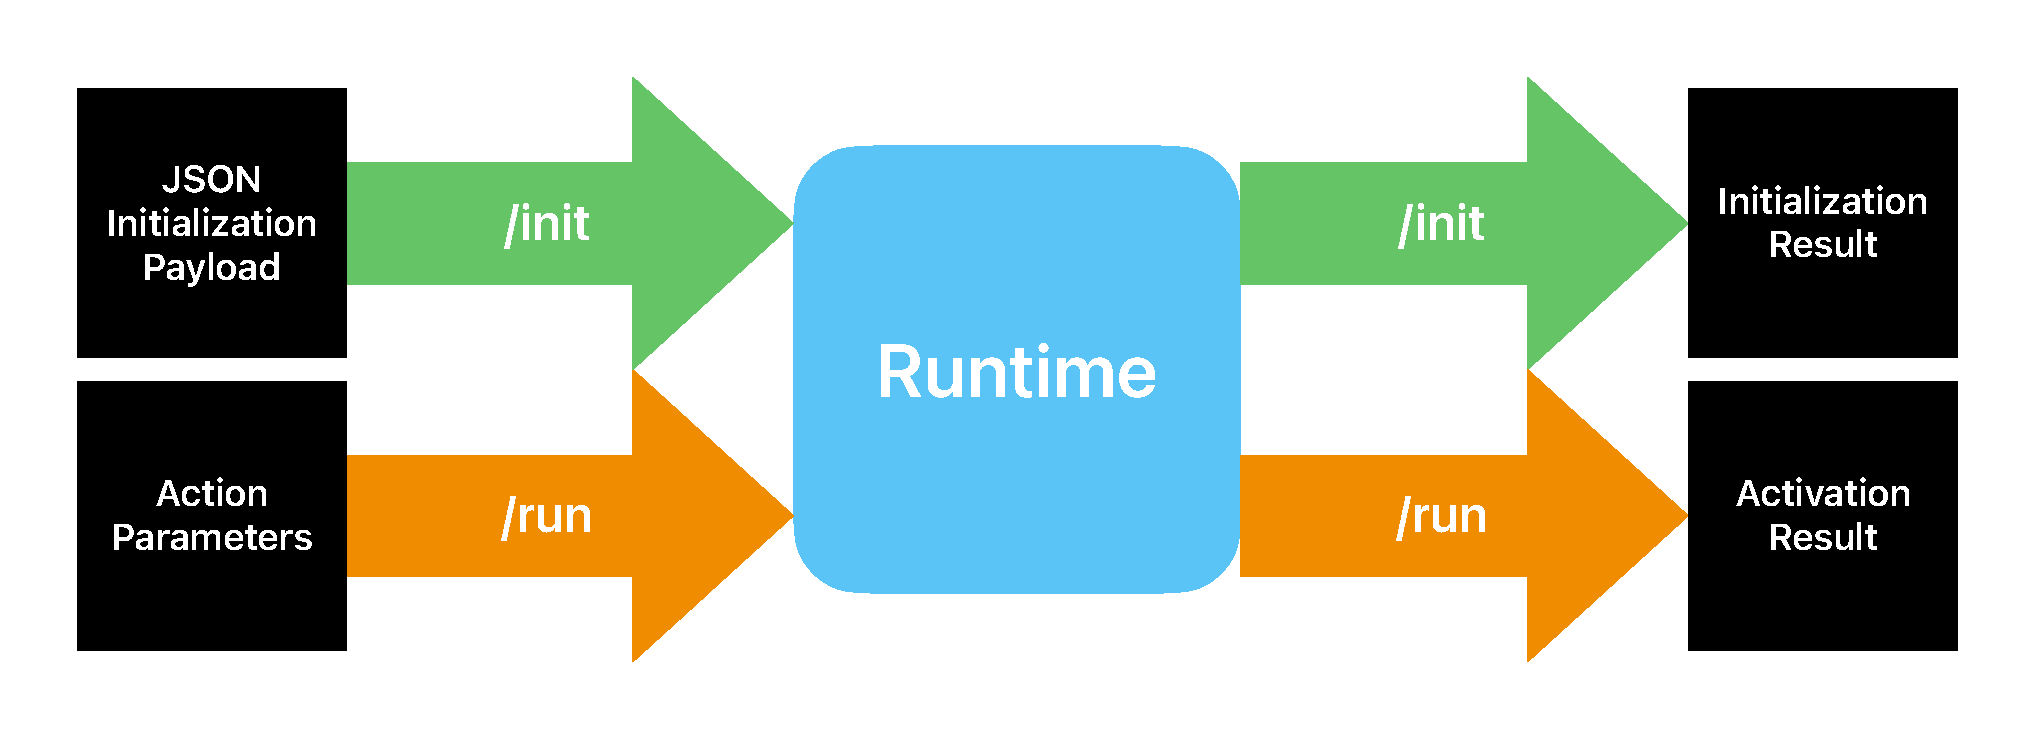
\includegraphics[width=\textwidth]{media/action_interface.pdf}
    \caption{Abstract representation of the Action Interface in OpenWhisk.}
    \label{fig:actioninterface}
\end{figure}

In OpenWhisk, the proxy functions as a web server, exposing two endpoints on port 8080: /init and /run. The /init endpoint is tasked with container initialization and accepts a POST request consisting of a JSON object that includes the action name, function to be executed, the source code, and several environment variables. This initialization happens exactly once and must be completed within a predefined time limit set by the platform \cite{openwhisk2023}.

Once initialization is completed successfully, the proxy transitions to a state where it can activate the function. The /run endpoint is responsible for this task. It receives an HTTP POST request with a new activation context and the function's input parameters. The route needs to accept a JSON object and respond with one, adhering to the OpenWhisk platform's prescribed schema. Every action in OpenWhisk has a set time limit, within which the activation must complete. If the function executes successfully, the route responds with 200 OK, and the response body is recorded as the result of the activation \cite{openwhisk2023}.

Moreover, logging is an integral part of the proxy's functionality. It flushes all the logs generated during initialization and execution, adding a unique frame marker at the end of each activation log stream. This marker is necessary to avoid delayed or truncated activation logs \cite{openwhisk2021}.

\subsection{ActionLoop Proxy in OpenWhisk}

The ActionLoop proxy is a tool designed to simplify the process of creating new OpenWhisk runtimes. While one can develop a new runtime by following the OpenWhisk runtime specification, the ActionLoop proxy offers a quicker and more efficient way to achieve this by implementing most of the specification out-of-the-box \cite{openwhisk2023}.

The ActionLoop proxy is a runtime engine, developed in Go, initially designed to support the OpenWhisk Go language runtime. However, its generic design allows it to be adapted for other language runtimes such as Swift, PHP, Python, Rust, Java, Ruby, and Crystal. It was engineered keeping both compiled and scripting languages in mind \cite{openwhisk2023}.

Using the ActionLoop proxy, one can develop a new runtime in a fraction of the time it would take to create one from scratch. This is due to the fact that the ActionLoop proxy requires the developer to write only a command line protocol instead of a full-fledged web server, reducing complexity. Additionally, the ActionLoop proxy is known to significantly enhance the performance of existing runtimes, providing speed improvements ranging from 2x to 20x \cite{openwhisk2023}.

In our work, we leverage the ActionLoop proxy to update the OpenWhisk runtime to support the latest version of Swift, enhancing the potential for Swift to be used as a Serverless language.

\section{Overview of the officially supported Swift runtime in OpenWhisk}
Apache OpenWhisk supports a variety of programming languages for writing actions, through the use of specific runtimes. As per the official documentation, the following runtimes are currently supported 
~\cite{openwhisk2023}:

\begin{itemize}
\item .Net: OpenWhisk runtime for .Net Core 2.2.
\item Go: OpenWhisk runtime for Go.
\item Java: OpenWhisk runtime for Java 8 (OpenJDK 8, JVM OpenJ9).
\item JavaScript: OpenWhisk runtime for Node.js v10, v12, and v14.
\item PHP: OpenWhisk runtime for PHP 8.0, 7.4, and 7.3.
\item Python: OpenWhisk runtime for Python 2.7, 3, and a 3 runtime variant for AI/ML (including packages for Tensorflow and PyTorch).
\item Ruby: OpenWhisk runtime for Ruby 2.5.
\item Swift: OpenWhisk runtime for Swift 3.1.1, 4.1, and 4.2.
\end{itemize}

These runtimes are officially released by the Apache OpenWhisk project and made available on the OpenWhisk Downloads page.

\section{Benefits of newer Swift features for serverless computing}
% Content here, such as async/await

\section{Challenges faced while updating the runtime}
% General challenges content here

\subsection{Understanding the current runtime architecture}
% Content about understanding the current architecture

\subsection{Implementing support for the latest Swift version (5.8)}
% Content about implementing support for Swift 5.8

\section{Steps to update the Swift runtime in OpenWhisk}
% General steps content here

\subsection{Description of the process and tools required}
% Content about the process and required tools

\subsection{Code snippets and configuration changes for updating the runtime}
% Content about code snippets and configuration changes, use listings or any other preferred package for code snippets

\section{Verifying the updated runtime functionality}
% General content about verifying the updated runtime

\subsection{Testing and validating the new runtime with the synchronization system case study}
% Content about testing and validation with the case study

\section{Potential benefits and applications of the updated runtime for future researchers}
% Content about potential benefits and applications

\section{Possible further improvements or updates to the runtime}
% Content about possible improvements or updates to the runtime
